\subsection{First approach: Game Theory}

We propose to solve the resource allocation problem previously described using the formalism of Game Theory.
We consider a two player game, where one player will be the attacker and will compromise the infrastructure to gain access to confidential data. The other player will be the the infrastructure owner and will be referred to as ''the defender`` for the rest of this chapter.
We will present the assumptions made, the players, their strategies and the different types of games considered.

\subsubsection{Expected results from the games}
Regardless of the type of game considered, we investigated the game with the following idea in mind: "Can we minimize the burden of monitoring by using alternative strategies like decoys or Moving Target Defense ?".
The solution of the game is supposed to show whether or not the defender can benefit from these techniques, and in a similar way, how much scanning the attacker should do prior to attacking the infrastructure.



\subsubsection{Assumptions}
We have made several assumptions about the scope of the game:\\
\textbf{Migration: } The migration has already started when the game starts.\\
\textbf{Constrained budgets: } Both players have limited capacities to either attack or defend the infrastructure.
This implies that the whole infrastructure cannot be attacker or defended.\\
\textbf{Complete information: } The game is considered to be of complete information.\\


\subsubsection{Defender}
The goal of the defender is to protect his infrastructure by either deploying monitoring or decoy on nodes. A decoy node contains flow rules that will mislead the attacker into believing the node is part of the new embedding of the migrated network.

The defender can choose among three different strategies:\\
\textbf{Installing a decoy: } The defender installs flow rules in a node that will hold information related to the migrated network but the node will in fact not be used to embed the virtual network.\\
\textbf{Monitoring a node: } The defender deploys monitoring on the node to contribute to the detection.\\
\textbf{Doing nothing}

\subsubsection{Attacker}
The attacker will compromise the migration to gain access to his victim's sensitive data.
The attack is done by installing flow rules in specific nodes that will allow him to duplicate the victim's traffic towards one of his virtual machines, as depicted in Fig.~\ref{fig:data-exfiltration-attack}. 
The attacker will compromise several nodes in order to establish a path between his victim's VN and one of his VMs.
He will then use the compromised nodes to duplicate the victim's network traffic and redirect it towards his VM.
The attack is considered complete when all the nodes establishing the full unauthorized path have been compromised.

\textbf{Location: } The attacker has compromised one node in the infrastructure.\\
\textbf{Attacker's resources: } The attacker owns virtual machines in the infrastructure.\\
\textbf{Attacker's capacities: } The attacker can scan or attack any node in the infrastructure.\\
\textbf{Attacker's victim knowledge: } The attacker can identify the flow rules belonging to his victim.\\
\textbf{Attacker's infrastructure knowledge: } The attacker has the view of the whole physical infrastructure.\\
\textbf{Attacker's embedding knowledge: } The attacker does not know the new embedding for his victim's virtual network.


The attacker can choose among three different strategies:\\
\textbf{Scanning a node: } The attacker can request the list of  flow rules installed in a node. This allows him to discover the embedding location of his victim.\\
\textbf{Attacking a node: } The attacker will install in a node specific rules to construct the path between his VM and the victim's virtual network.\\
\textbf{Doing nothing}\\



\subsubsection{Games considered to solve the RA problem}
We have considered several types of games for this problem, and we will present their limitations and impact.

\textbf{Static games:} These games are played on each node of the infrastructure, only once. We investigated a game based on the works of Ismail~\etal~\cite{Chen2009,interdep-ismail2017}. The immediate limitation of this game is the inadequacy to use scans and decoys as the attacker is supposed to leverage the information collected to improve his next attack. This leaves us with a model where the attacker either attacks a node or not, and similarly the defender does the same.

The second limitation of static games is their inadequacy to represent the migration process as a succession of steps, where the system would become more and more worth attacking because the number of nodes holding valuable information would increase as the migration goes on.

% The work of Ismail~\etal takes the Game Theory formalism far in the modeling, and focuses on several aspects of an infrastructure running on a legacy network. The opportunity here is to add the representation of SDN and the decoupling of the control plane and the data plane in the model.

The previous limitations convinced us that static games were not a fruitful lead to investigate.
We draw the same conclusion for repeated games, as these are static games repeated several times without any change in the way the game is played.

% \textbf{Repeated games: } These games are static games played several times.
% Since the game must remain unchanged at every play, the limitations encountered woth static games still apply here. 

\textbf{Sequential games: } These games represent players taking turns choosing their action. This aspect makes them more interesting to consider than static games, because the migration process can be represented along the choices made by players. In this situation, the complete information aspect of the game can still be maintained, but the idea of using decoy in the infrastructure requires an imperfect information game. The location of decoys must remain unknown to the attacker to be effective.
Indeed, if the attacker knows where the decoys are deployed he will not attack these nodes.

The main limitation encountered here is that the choice of all players must be revealed after every player has chosen his strategy. Therefore, it is impossible to accumulate rounds without revealing the defender's actions to the attacker. This makes the use of decoys worthless and limit us again to a simple attack/defend/do nothing scheme, similarly to static games.

\textbf{Stochastic games:} Modeling the evolution of a system based on the choices made by players is an interesting formalism for our problem. We can consider the evolution of the infrastructure as the migration process goes on, as well as the progress of the attacker to exfiltrate the data. 

These costs are different for the attacker and the defender, thus making the game a non zero-sum stochastic game. Non zero sum stochastic games with imperfect information turn out to be widely complex to solve, and to the best of our knowledge there is no algorithm that can be used as a support for the resolution in a reasonable time. 
% The technical limitations we are faced with does not makes it worthwhile to consider such a complex model to be exploited in this thesis.


\subsubsection{Discussion}
We have reviewed several types of games in this section, where each game has its own share of limitations regarding our problem. Another aspect that we have not detailed before is the acceptable granularity of actions for the players. Indeed, the vast majority of work we have surveyed in Chapter~\ref{sec:sota} limit the players to a binary choice: attacking/defending or doing nothing. This reduced number of choices leaves us with the interrogation of whether we are allowed to define precise strategies for a security game, or if each strategy must be significantly different from every other~\cite{Kiennert2018}.% Finally, depending on the type of game chosen, the realism of the modeling is also heavily impacted because of the assumptions made about the system to protect.
% as well as the arbitrary choices made for the costs and rewards.
% In the state of the art, the values chosen in the utility functions rarely are evaluated using a real life methodology, especially on the attacker side where the literature is very scarce. 
This leaves us with the question: "Is the game we have formulated coherent and realistic with current real life use cases ?". 

We conclude this section with the observation that Game Theory does not offer enough flexibility to model our problem. In the next chapter, we explore the use of Markov Decision Processes and illustrate how this formalism can be used to include the consequences of attacks in the strategy of the defender.

\begin{figure*}[htbp]


\tikzset{every picture/.style={line width=0.75pt}} %set default line width to 0.75pt        

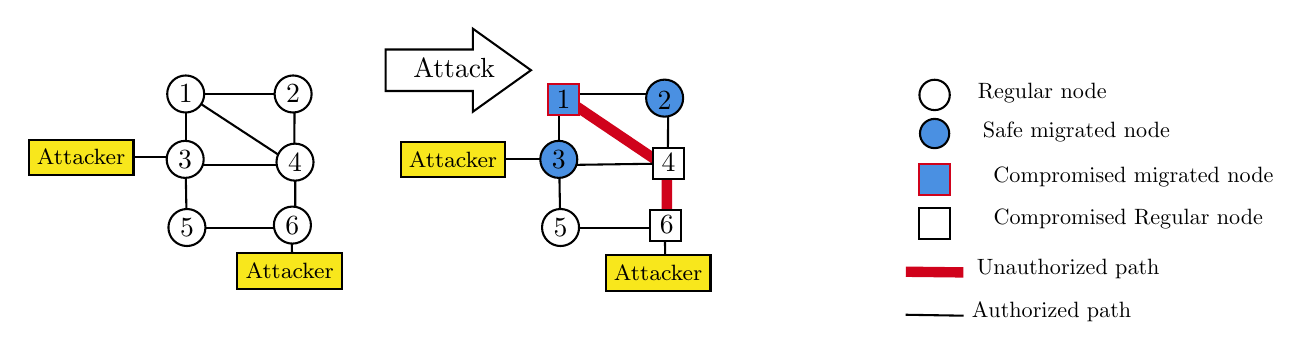
\begin{tikzpicture}[x=0.75pt,y=0.75pt,yscale=-1,xscale=1]
%uncomment if require: \path (0,300); %set diagram left start at 0, and has height of 300

%Straight Lines [id:da7739123357617682] 
\draw    (70.75,83.4) -- (108.67,83.4) ;


%Shape: Rectangle [id:dp46476407013383825] 
\draw  [fill={rgb, 255:red, 248; green, 231; blue, 28 }  ,fill opacity=1 ] (29.2,75.2) -- (79.67,75.2) -- (79.67,92.18) -- (29.2,92.18) -- cycle ;


%Straight Lines [id:da13064923443841459] 
\draw    (249.95,84.6) -- (287.87,84.6) ;


%Shape: Rectangle [id:dp28554238318371994] 
\draw  [fill={rgb, 255:red, 248; green, 231; blue, 28 }  ,fill opacity=1 ] (208.4,76.4) -- (258.87,76.4) -- (258.87,93.38) -- (208.4,93.38) -- cycle ;


%Straight Lines [id:da567285896843154] 
\draw [color={rgb, 255:red, 208; green, 2; blue, 27 }  ,draw opacity=1 ][line width=3.75]    (336.65,85.21) -- (336.67,119) ;


%Straight Lines [id:da046576842172091903] 
\draw [color={rgb, 255:red, 208; green, 2; blue, 27 }  ,draw opacity=1 ][line width=3.75]    (290.52,57.47) -- (333.33,86.33) ;


%Straight Lines [id:da5668243278416182] 
\draw    (157.33,49.22) -- (157.17,80.81) ;


%Straight Lines [id:da49434419911731065] 
\draw    (111.08,117.73) -- (149,117.73) ;


%Straight Lines [id:da6673139716829495] 
\draw    (155.58,114.06) -- (156.5,144) ;


%Straight Lines [id:da9840681038768349] 
\draw    (104.83,53.23) -- (160.58,89.73) ;


%Straight Lines [id:da4482722852442499] 
\draw    (104.83,89.73) -- (105.33,117.55) ;


%Straight Lines [id:da7670268694366985] 
\draw    (157.58,87.73) -- (157.67,119.88) ;


%Shape: Circle [id:dp667695613861877] 
\draw  [fill={rgb, 255:red, 255; green, 255; blue, 255 }  ,fill opacity=1 ] (95.92,53.23) .. controls (95.92,48.3) and (99.91,44.31) .. (104.83,44.31) .. controls (109.76,44.31) and (113.75,48.3) .. (113.75,53.23) .. controls (113.75,58.15) and (109.76,62.15) .. (104.83,62.15) .. controls (99.91,62.15) and (95.92,58.15) .. (95.92,53.23) -- cycle ;

%Shape: Circle [id:dp7262621996740888] 
\draw  [fill={rgb, 255:red, 255; green, 255; blue, 255 }  ,fill opacity=1 ] (148.58,86.06) .. controls (148.58,81.14) and (152.58,77.15) .. (157.5,77.15) .. controls (162.42,77.15) and (166.42,81.14) .. (166.42,86.06) .. controls (166.42,90.99) and (162.42,94.98) .. (157.5,94.98) .. controls (152.58,94.98) and (148.58,90.99) .. (148.58,86.06) -- cycle ;

%Shape: Circle [id:dp08856327459465119] 
\draw  [fill={rgb, 255:red, 255; green, 255; blue, 255 }  ,fill opacity=1 ] (147.33,116.4) .. controls (147.33,111.47) and (151.33,107.48) .. (156.25,107.48) .. controls (161.17,107.48) and (165.17,111.47) .. (165.17,116.4) .. controls (165.17,121.32) and (161.17,125.31) .. (156.25,125.31) .. controls (151.33,125.31) and (147.33,121.32) .. (147.33,116.4) -- cycle ;

%Straight Lines [id:da658208744911517] 
\draw    (113.75,53.23) -- (151.67,53.23) ;


%Straight Lines [id:da49379806707152474] 
\draw    (110.75,87.4) -- (148.67,87.4) ;


%Straight Lines [id:da6945831753833721] 
\draw    (104.83,62.15) -- (104.83,80.81) ;


%Shape: Circle [id:dp7034065447291917] 
\draw  [fill={rgb, 255:red, 255; green, 255; blue, 255 }  ,fill opacity=1 ] (96.52,117.56) .. controls (96.52,112.64) and (100.51,108.65) .. (105.43,108.65) .. controls (110.36,108.65) and (114.35,112.64) .. (114.35,117.56) .. controls (114.35,122.49) and (110.36,126.48) .. (105.43,126.48) .. controls (100.51,126.48) and (96.52,122.49) .. (96.52,117.56) -- cycle ;

%Shape: Circle [id:dp4778597289311547] 
\draw  [fill={rgb, 255:red, 255; green, 255; blue, 255 }  ,fill opacity=1 ] (95.67,84.73) .. controls (95.67,79.8) and (99.66,75.81) .. (104.58,75.81) .. controls (109.51,75.81) and (113.5,79.8) .. (113.5,84.73) .. controls (113.5,89.65) and (109.51,93.65) .. (104.58,93.65) .. controls (99.66,93.65) and (95.67,89.65) .. (95.67,84.73) -- cycle ;

%Shape: Circle [id:dp08437409893269954] 
\draw  [fill={rgb, 255:red, 255; green, 255; blue, 255 }  ,fill opacity=1 ] (147.67,53.23) .. controls (147.67,48.3) and (151.66,44.31) .. (156.58,44.31) .. controls (161.51,44.31) and (165.5,48.3) .. (165.5,53.23) .. controls (165.5,58.15) and (161.51,62.15) .. (156.58,62.15) .. controls (151.66,62.15) and (147.67,58.15) .. (147.67,53.23) -- cycle ;

%Shape: Circle [id:dp2544455966731902] 
\draw  [fill={rgb, 255:red, 74; green, 144; blue, 226 }  ,fill opacity=1 ] (458.61,72.28) .. controls (458.61,68.39) and (461.76,65.23) .. (465.66,65.23) .. controls (469.55,65.23) and (472.71,68.39) .. (472.71,72.28) .. controls (472.71,76.18) and (469.55,79.33) .. (465.66,79.33) .. controls (461.76,79.33) and (458.61,76.18) .. (458.61,72.28) -- cycle ;
%Straight Lines [id:da3025029961647492] 
\draw [color={rgb, 255:red, 208; green, 2; blue, 27 }  ,draw opacity=1 ][line width=3.75]    (451.78,138.87) -- (479.53,139.19) ;


%Shape: Circle [id:dp2181751678296382] 
\draw  [fill={rgb, 255:red, 255; green, 255; blue, 255 }  ,fill opacity=1 ] (458.35,53.69) .. controls (458.35,49.65) and (461.62,46.37) .. (465.66,46.37) .. controls (469.7,46.37) and (472.97,49.65) .. (472.97,53.69) .. controls (472.97,57.73) and (469.7,61) .. (465.66,61) .. controls (461.62,61) and (458.35,57.73) .. (458.35,53.69) -- cycle ;
%Straight Lines [id:da9324723367639798] 
\draw [color={rgb, 255:red, 0; green, 0; blue, 0 }  ,draw opacity=1 ]   (451.64,159.59) -- (479.68,160.05) ;


%Shape: Square [id:dp642864286437786] 
\draw  [color={rgb, 255:red, 208; green, 2; blue, 27 }  ,draw opacity=1 ][fill={rgb, 255:red, 74; green, 144; blue, 226 }  ,fill opacity=1 ] (458.16,86.93) -- (473.16,86.93) -- (473.16,101.93) -- (458.16,101.93) -- cycle ;
%Shape: Square [id:dp6103038230457687] 
\draw  [fill={rgb, 255:red, 255; green, 255; blue, 255 }  ,fill opacity=1 ] (458.16,108.16) -- (473.16,108.16) -- (473.16,123.16) -- (458.16,123.16) -- cycle ;

%Right Arrow [id:dp9004425172478334] 
\draw  [fill={rgb, 255:red, 255; green, 255; blue, 255 }  ,fill opacity=1 ] (201.2,31.78) -- (243.2,31.78) -- (243.2,21.78) -- (271.2,41.78) -- (243.2,61.78) -- (243.2,51.78) -- (201.2,51.78) -- cycle ;

%Straight Lines [id:da8396173497547912] 
\draw    (337.33,49.22) -- (337.17,80.81) ;


%Straight Lines [id:da9182383261146002] 
\draw    (291.08,117.73) -- (329,117.73) ;


%Straight Lines [id:da858414453735221] 
\draw    (335.58,114.06) -- (336,140.5) ;


%Straight Lines [id:da20295515063433045] 
\draw    (284.83,89.73) -- (285.33,117.55) ;


%Straight Lines [id:da24824224288757746] 
\draw    (293.75,53.23) -- (331.67,53.23) ;


%Straight Lines [id:da32113645413312253] 
\draw    (290.75,87.4) -- (337.58,86.73) ;


%Straight Lines [id:da20280015358357328] 
\draw    (284.83,62.15) -- (284.83,80.81) ;


%Shape: Circle [id:dp2078999158258219] 
\draw  [fill={rgb, 255:red, 255; green, 255; blue, 255 }  ,fill opacity=1 ] (276.52,117.56) .. controls (276.52,112.64) and (280.51,108.65) .. (285.43,108.65) .. controls (290.36,108.65) and (294.35,112.64) .. (294.35,117.56) .. controls (294.35,122.49) and (290.36,126.48) .. (285.43,126.48) .. controls (280.51,126.48) and (276.52,122.49) .. (276.52,117.56) -- cycle ;

%Shape: Circle [id:dp17283437144421832] 
\draw  [fill={rgb, 255:red, 74; green, 144; blue, 226 }  ,fill opacity=1 ] (275.67,84.73) .. controls (275.67,79.8) and (279.66,75.81) .. (284.58,75.81) .. controls (289.51,75.81) and (293.5,79.8) .. (293.5,84.73) .. controls (293.5,89.65) and (289.51,93.65) .. (284.58,93.65) .. controls (279.66,93.65) and (275.67,89.65) .. (275.67,84.73) -- cycle ;

%Shape: Circle [id:dp6292985525556183] 
\draw  [fill={rgb, 255:red, 74; green, 144; blue, 226 }  ,fill opacity=1 ] (326.67,55.23) .. controls (326.67,50.3) and (330.66,46.31) .. (335.58,46.31) .. controls (340.51,46.31) and (344.5,50.3) .. (344.5,55.23) .. controls (344.5,60.15) and (340.51,64.15) .. (335.58,64.15) .. controls (330.66,64.15) and (326.67,60.15) .. (326.67,55.23) -- cycle ;

%Shape: Square [id:dp21738038837827933] 
\draw  [color={rgb, 255:red, 208; green, 2; blue, 27 }  ,draw opacity=1 ][fill={rgb, 255:red, 74; green, 144; blue, 226 }  ,fill opacity=1 ] (279.37,48.2) -- (294.37,48.2) -- (294.37,63.2) -- (279.37,63.2) -- cycle ;
%Shape: Square [id:dp8476679341444072] 
\draw  [fill={rgb, 255:red, 255; green, 255; blue, 255 }  ,fill opacity=1 ] (330.08,79.23) -- (345.08,79.23) -- (345.08,94.23) -- (330.08,94.23) -- cycle ;

%Shape: Square [id:dp8795975156412624] 
\draw  [fill={rgb, 255:red, 255; green, 255; blue, 255 }  ,fill opacity=1 ] (328.48,109.23) -- (343.48,109.23) -- (343.48,124.23) -- (328.48,124.23) -- cycle ;
%Shape: Rectangle [id:dp2088885864598815] 
\draw  [fill={rgb, 255:red, 248; green, 231; blue, 28 }  ,fill opacity=1 ] (129.7,130) -- (180.17,130) -- (180.17,146.98) -- (129.7,146.98) -- cycle ;

%Shape: Rectangle [id:dp5309747919784684] 
\draw  [fill={rgb, 255:red, 248; green, 231; blue, 28 }  ,fill opacity=1 ] (307.2,131) -- (357.67,131) -- (357.67,147.98) -- (307.2,147.98) -- cycle ;


% Text Node
\draw (336.65,116) node  [align=left] {6};
% Text Node
\draw (286.87,55.7) node  [align=left] {1};
% Text Node
\draw (332.44,139.49) node  [align=left] {{\footnotesize Attacker}};
% Text Node
\draw (154.94,138.49) node  [align=left] {{\footnotesize Attacker}};
% Text Node
\draw (337.5,86.06) node  [align=left] {4};
% Text Node
\draw (335.58,56.23) node  [align=left] {2};
% Text Node
\draw (284.58,84.73) node  [align=left] {3};
% Text Node
\draw (285.43,117.56) node  [align=left] {5};
% Text Node
\draw (234.2,40.8) node  [align=left] {Attack};
% Text Node
\draw (522,158.05) node [scale=0.8] [align=left] {Authorized path};
% Text Node
\draw (530,137.33) node [scale=0.8] [align=left] {Unauthorized path};
% Text Node
\draw (559,113.58) node [scale=0.8] [align=left] {Compromised Regular node};
% Text Node
\draw (561.5,93.17) node [scale=0.8] [align=left] {Compromised migrated node};
% Text Node
\draw (534,71.48) node [scale=0.8] [align=left] {Safe migrated node};
% Text Node
\draw (517.5,52.62) node [scale=0.8] [align=left] {Regular node};
% Text Node
\draw (156.58,53.23) node  [align=left] {2};
% Text Node
\draw (104.58,84.73) node  [align=left] {3};
% Text Node
\draw (105.43,117.56) node  [align=left] {5};
% Text Node
\draw (156.25,116.4) node  [align=left] {6};
% Text Node
\draw (157.5,86.06) node  [align=left] {4};
% Text Node
\draw (104.83,53.23) node  [align=left] {1};
% Text Node
\draw (233.64,84.89) node  [align=left] {{\footnotesize Attacker}};
% Text Node
\draw (54.44,83.69) node  [align=left] {{\footnotesize Attacker}};


\end{tikzpicture}



\caption{Exfiltrating information via unauthorized routing}
\label{fig:data-exfiltration-attack}
\end{figure*}

